\section{RL as ``Universal'' Learning}

% ---------------------------------------------------------------- Slide 57 (divider)
\begin{frame}{}
    \LARGE Reinforcement Learning as \textbf{``Universal'' Learning}
\end{frame}

% ---------------------------------------------------------------- Slide 58
\begin{frame}{Large-scale machine learning}
\centering
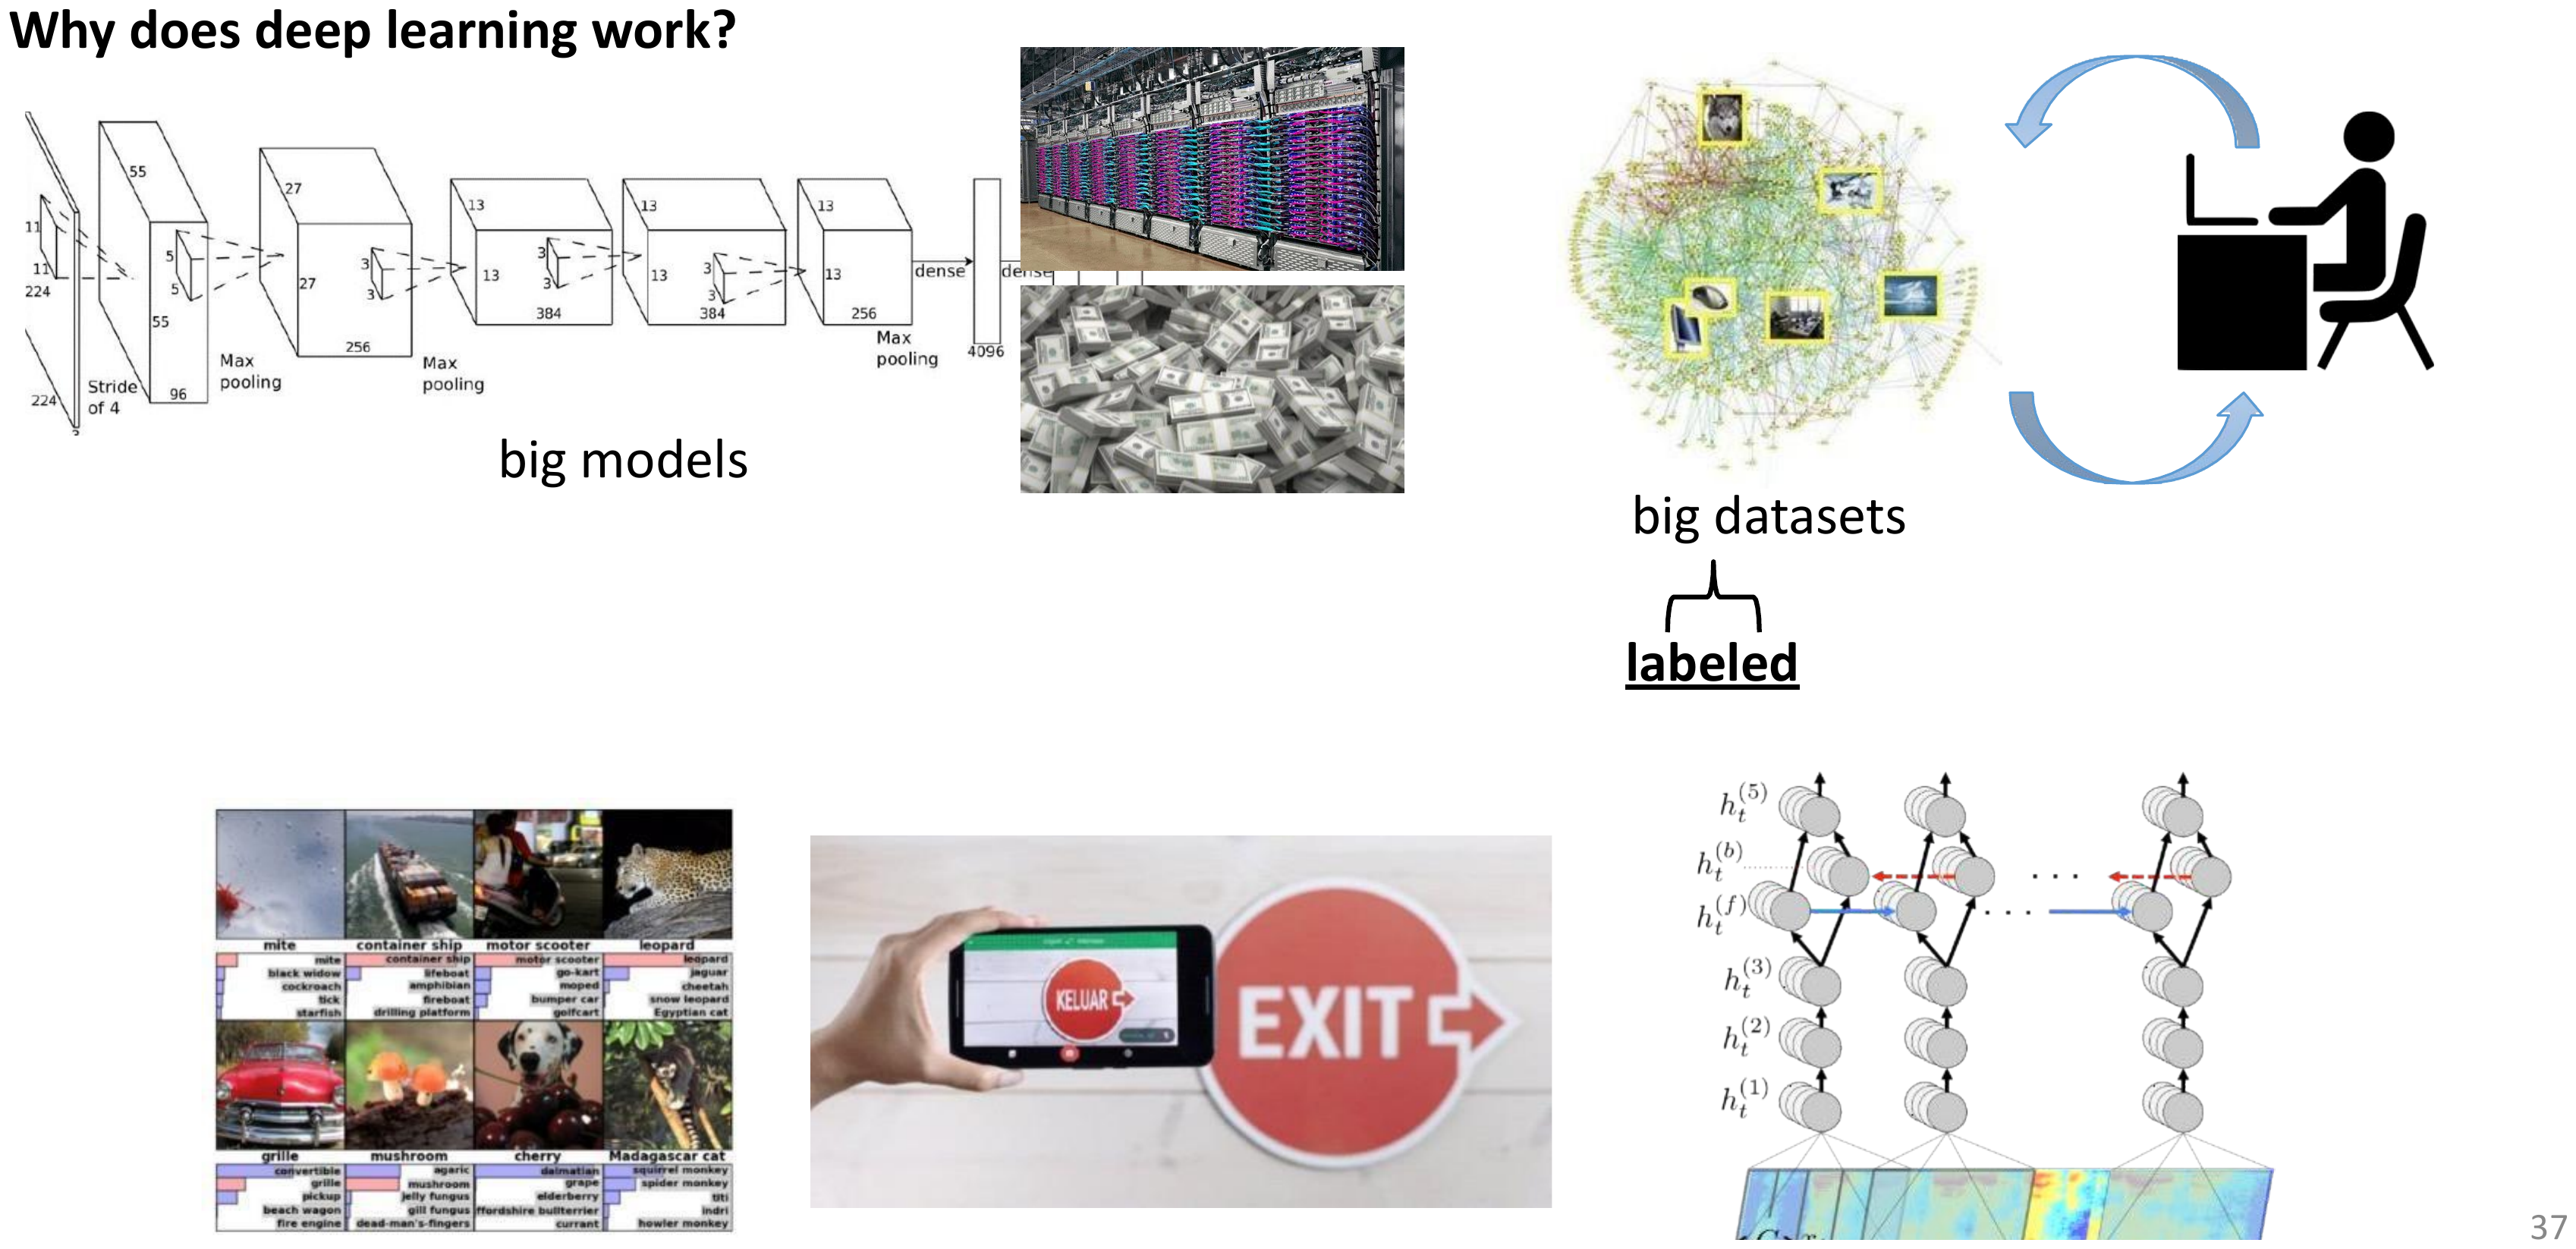
\includegraphics[width=\linewidth,height=0.84\textheight,keepaspectratio]{images/meta-rl-open/figures/largescale-full.png}
\end{frame}

% ---------------------------------------------------------------- Slide 59
\begin{frame}{Reducing the supervision burden}
\centering
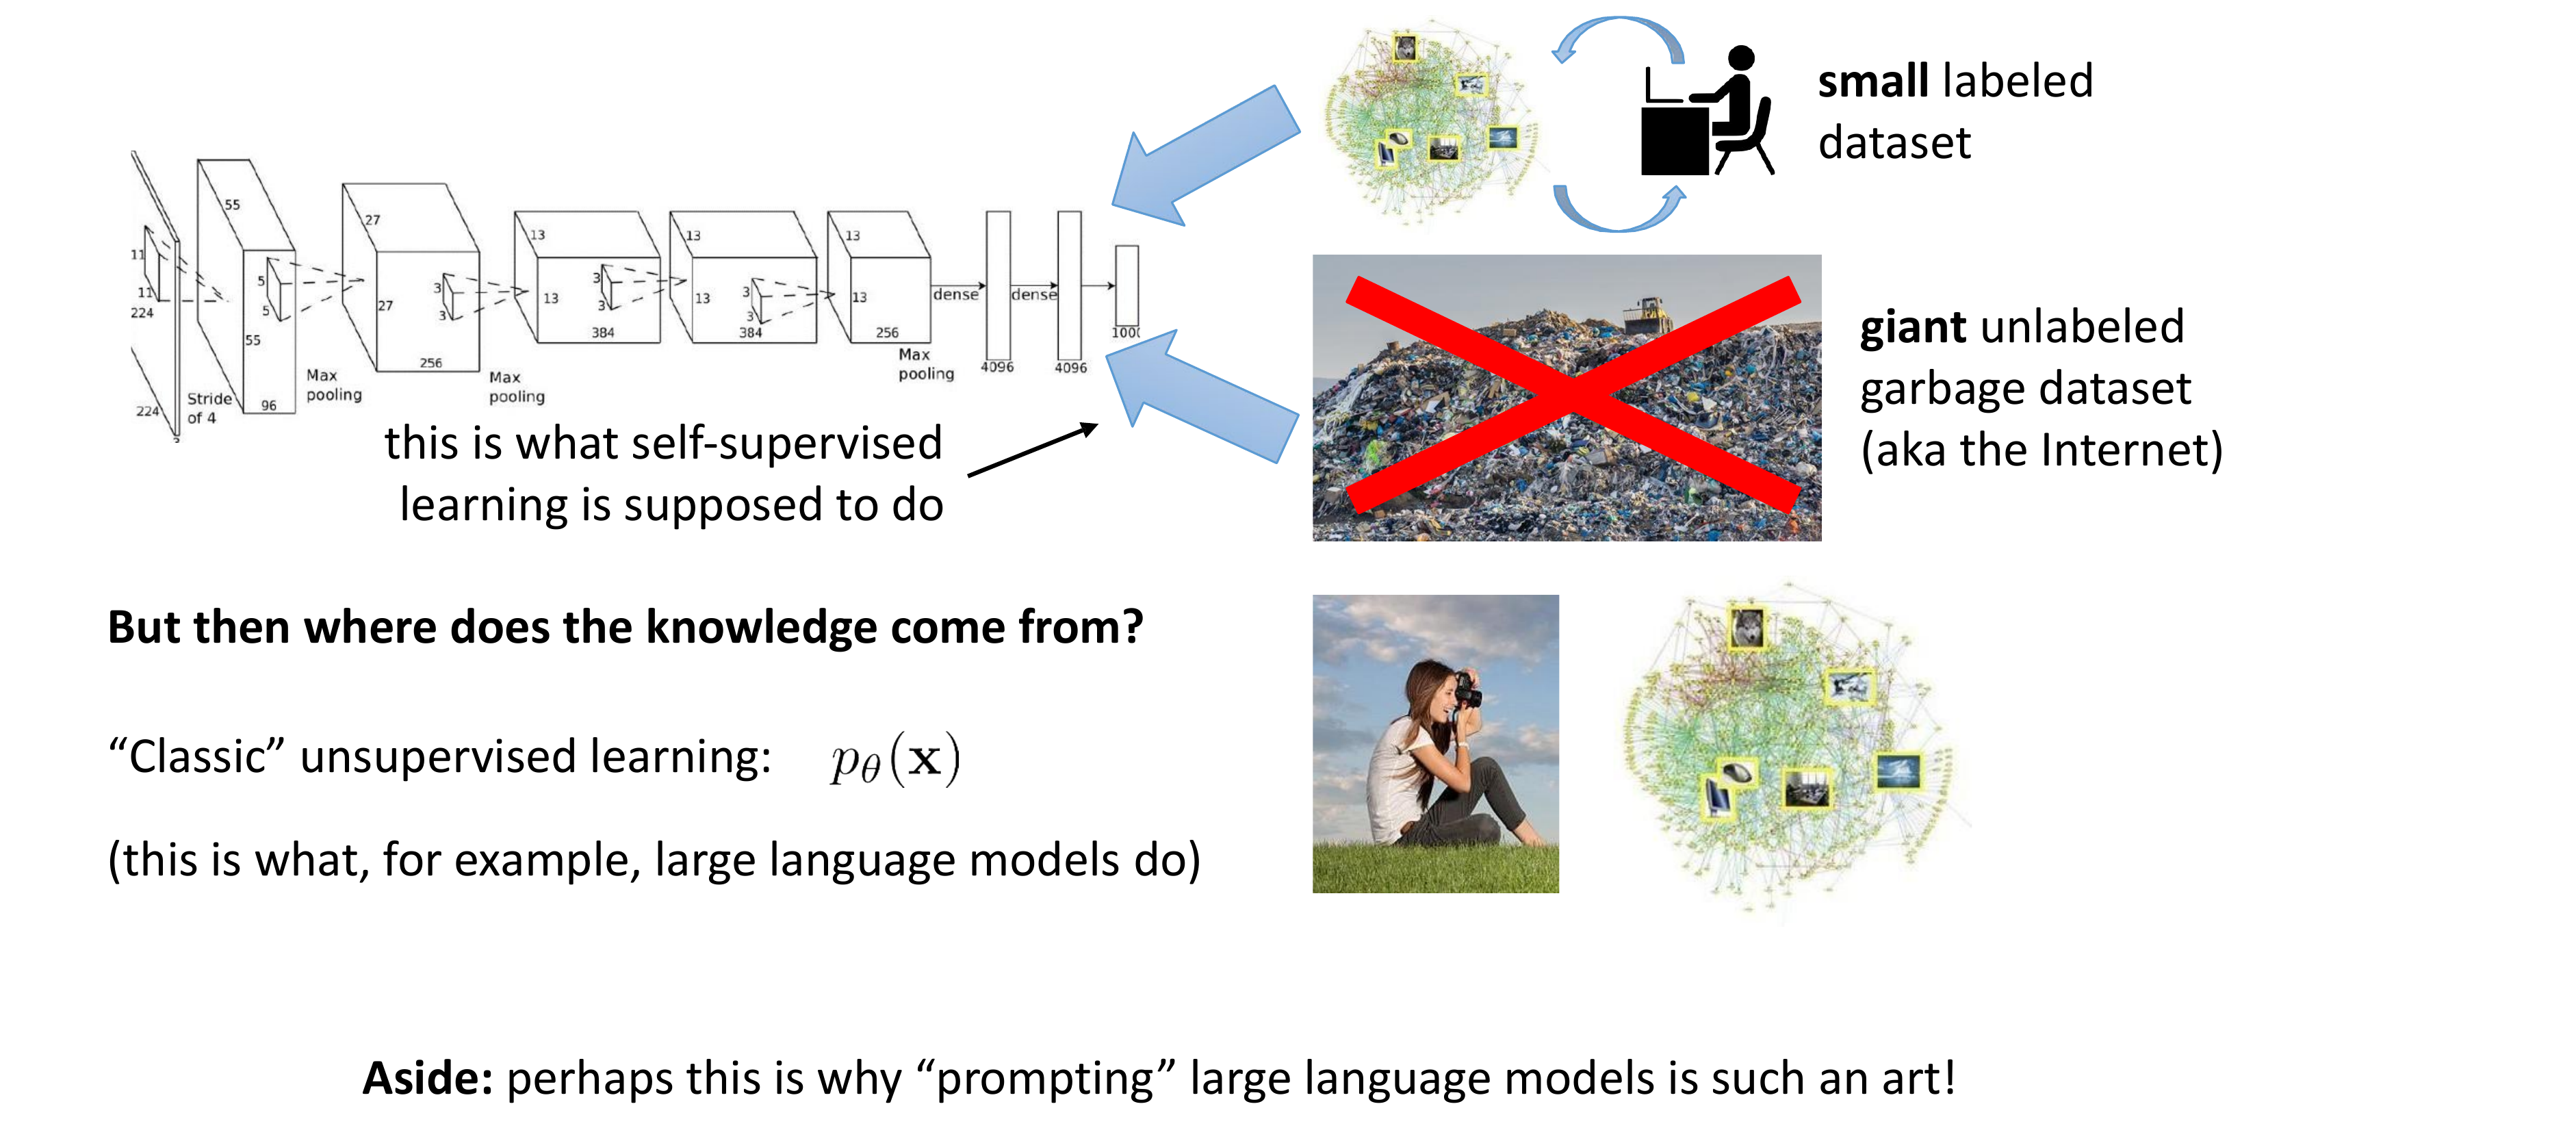
\includegraphics[width=\linewidth,height=0.84\textheight,keepaspectratio]{images/meta-rl-open/figures/reducing-full.png}
\end{frame}

% ---------------------------------------------------------------- Slide 60
\begin{frame}{Stepping back a bit\dots}
\begin{columns}[c]
\begin{column}{0.56\textwidth}
\footnotesize
Why do we need \textbf{machine learning} anyway?
\vspace{0.4em}

{\setlength{\fboxsep}{4pt}%
\fcolorbox{red}{white}{\begin{minipage}{0.95\linewidth}
\textbf{A postulate:} We need machine learning for one reason and one reason only ---
that's to produce \textbf{\underline{adaptable and complex decisions}}.
\end{minipage}}}
\vspace{0.5em}

\newcommand{\declined}[2]{\raisebox{-0.45\height}{\includegraphics[height=0.85cm]{images/meta-rl-open/figures/#1}}\;\; #2}

\declined{ml-robot.jpg}{Decision: how do I move my joints?}\par\vspace{0.3em}
\declined{ml-car.jpg}{Decision: how do I steer the car?}\par\vspace{0.3em}
\declined{ml-imagenet.jpg}{What is the decision? The image label? {\color{red}\textbf{Usually not!}}}\par\vspace{0.3em}
What happens with that label afterwards? \emph{These are {\color{red}\textbf{decisions}} ---
they lead to {\color{red}\textbf{consequences}}}
\end{column}
\begin{column}{0.42\textwidth}
\footnotesize
\textbf{Aside:} why do we need \textbf{brains} anyway?

\vspace{0.4em}
\colorbox{blue!6}{%
\begin{minipage}{0.94\linewidth}
\centering
\begin{minipage}{0.34\linewidth}\centering
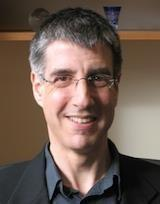
\includegraphics[width=\linewidth]{images/meta-rl-open/figures/wolpert-photo.jpg}\\[0.2em]
{\scriptsize\textbf{Daniel Wolpert}}\\
{\tiny (knows quite a lot about brains)}
\end{minipage}\hfill
\begin{minipage}{0.32\linewidth}\centering

\includegraphics[width=\linewidth]{images/meta-rl-open/figures/brain-icon.jpg}
\end{minipage}

\vspace{0.5em}
{\scriptsize\itshape ``We have a brain for one reason and one reason only --- that's to
produce \textbf{adaptable and complex movements}. Movement is the only way we have
affecting the world around us\dots I believe that to understand movement is to understand
the whole brain.''}
\end{minipage}}
\end{column}
\end{columns}
\end{frame}

% ---------------------------------------------------------------- Slide 61
\begin{frame}{Reinforcement learning as a way to use ``cheap'' data}
\centering
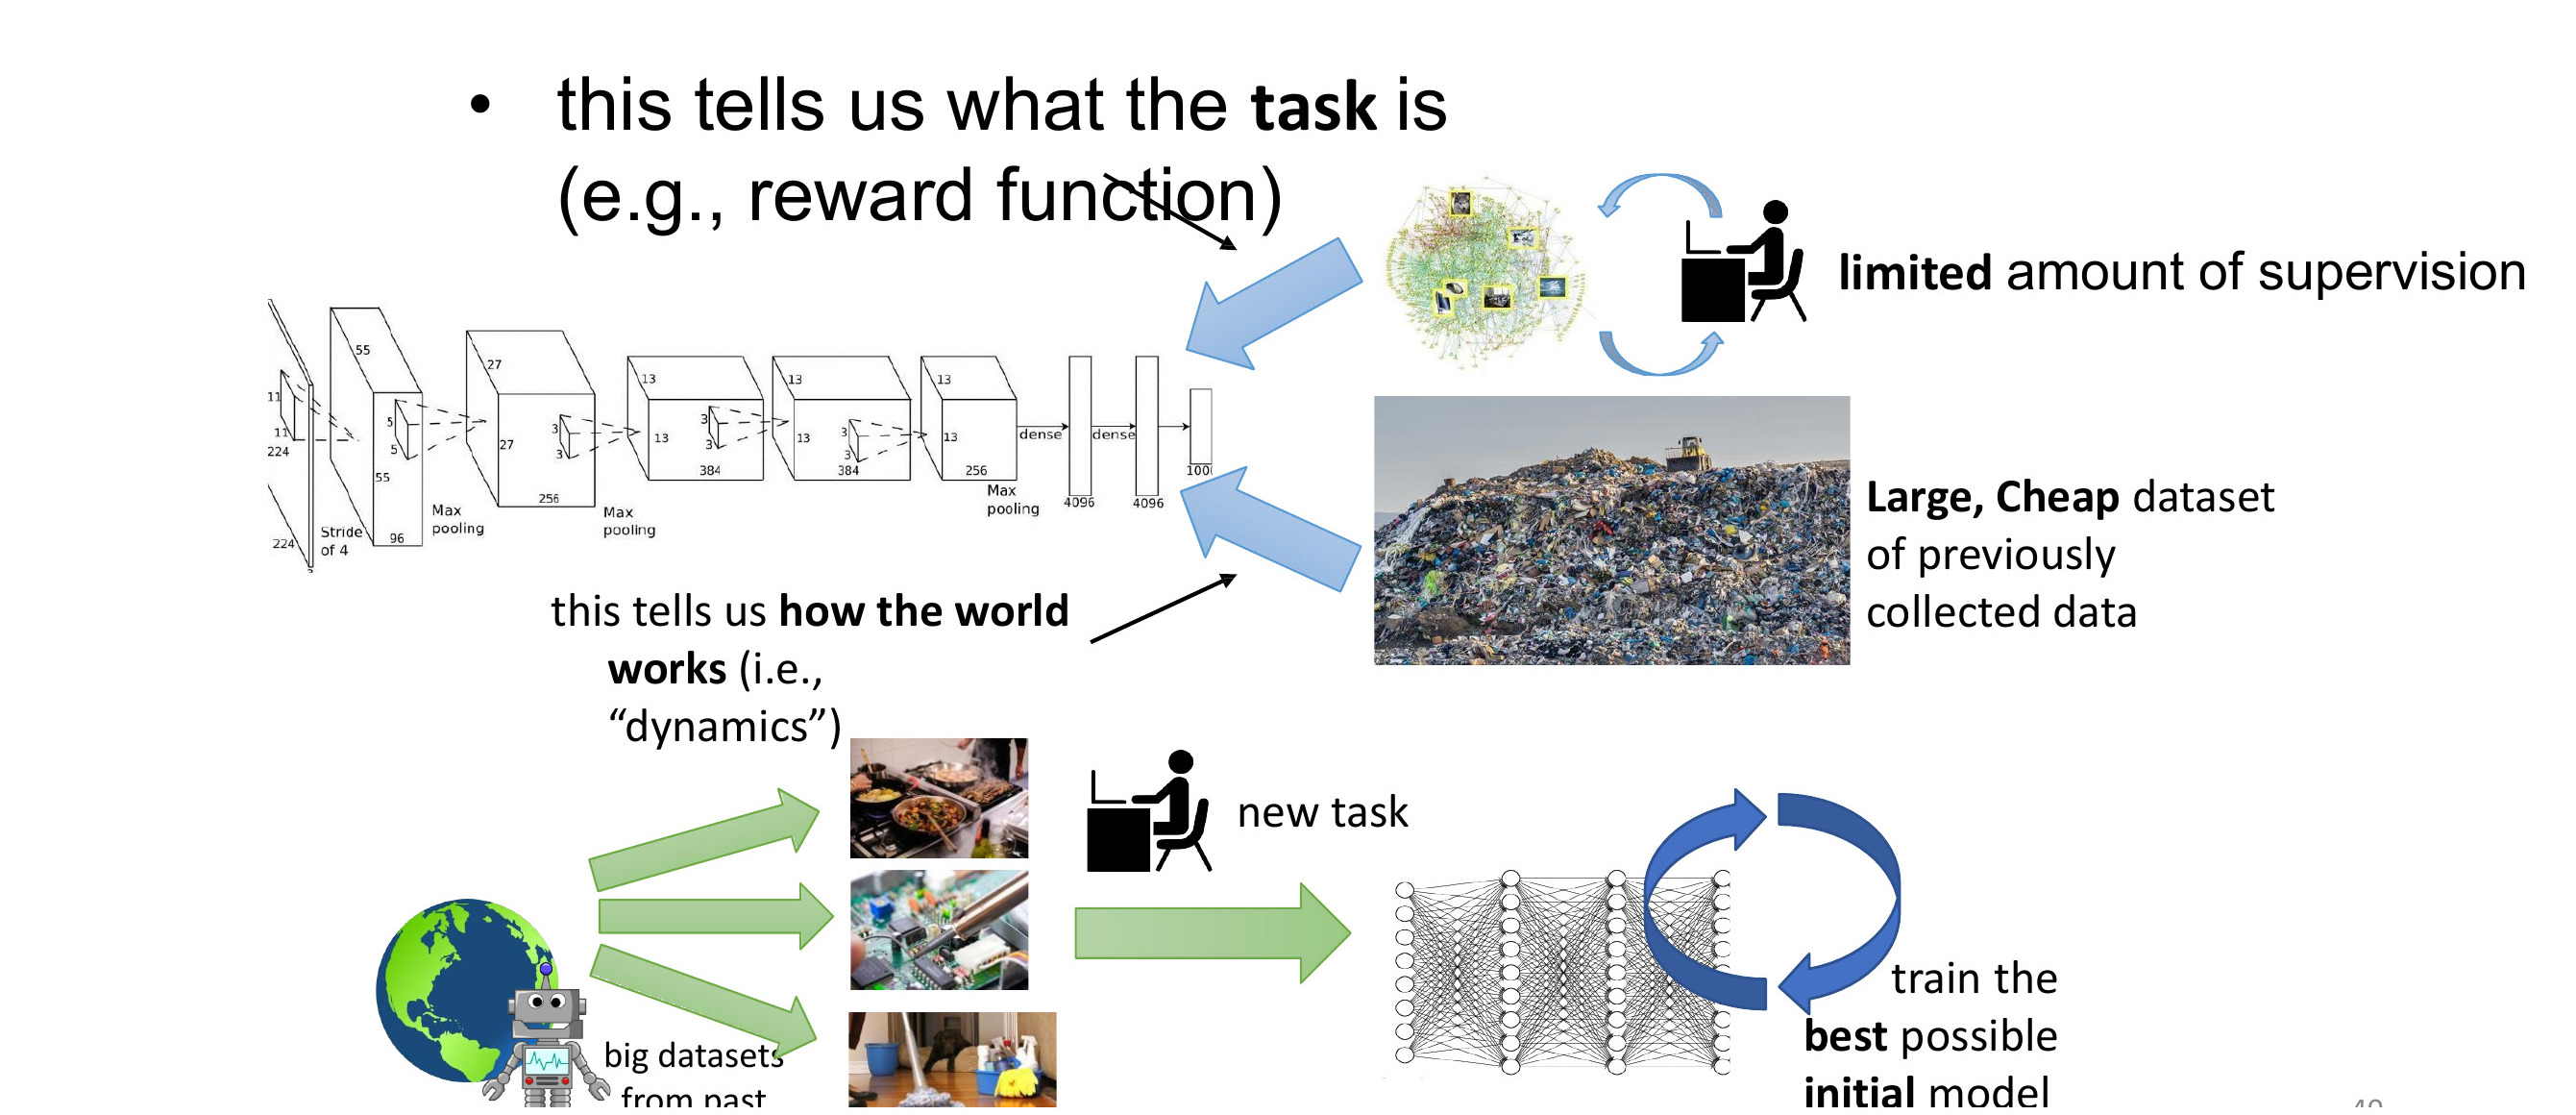
\includegraphics[width=\linewidth,height=0.82\textheight,keepaspectratio]{images/meta-rl-open/figures/cheap-data.jpg}
\end{frame}

% ---------------------------------------------------------------- Slide 62
\begin{frame}{The RL + data problem}
\centering
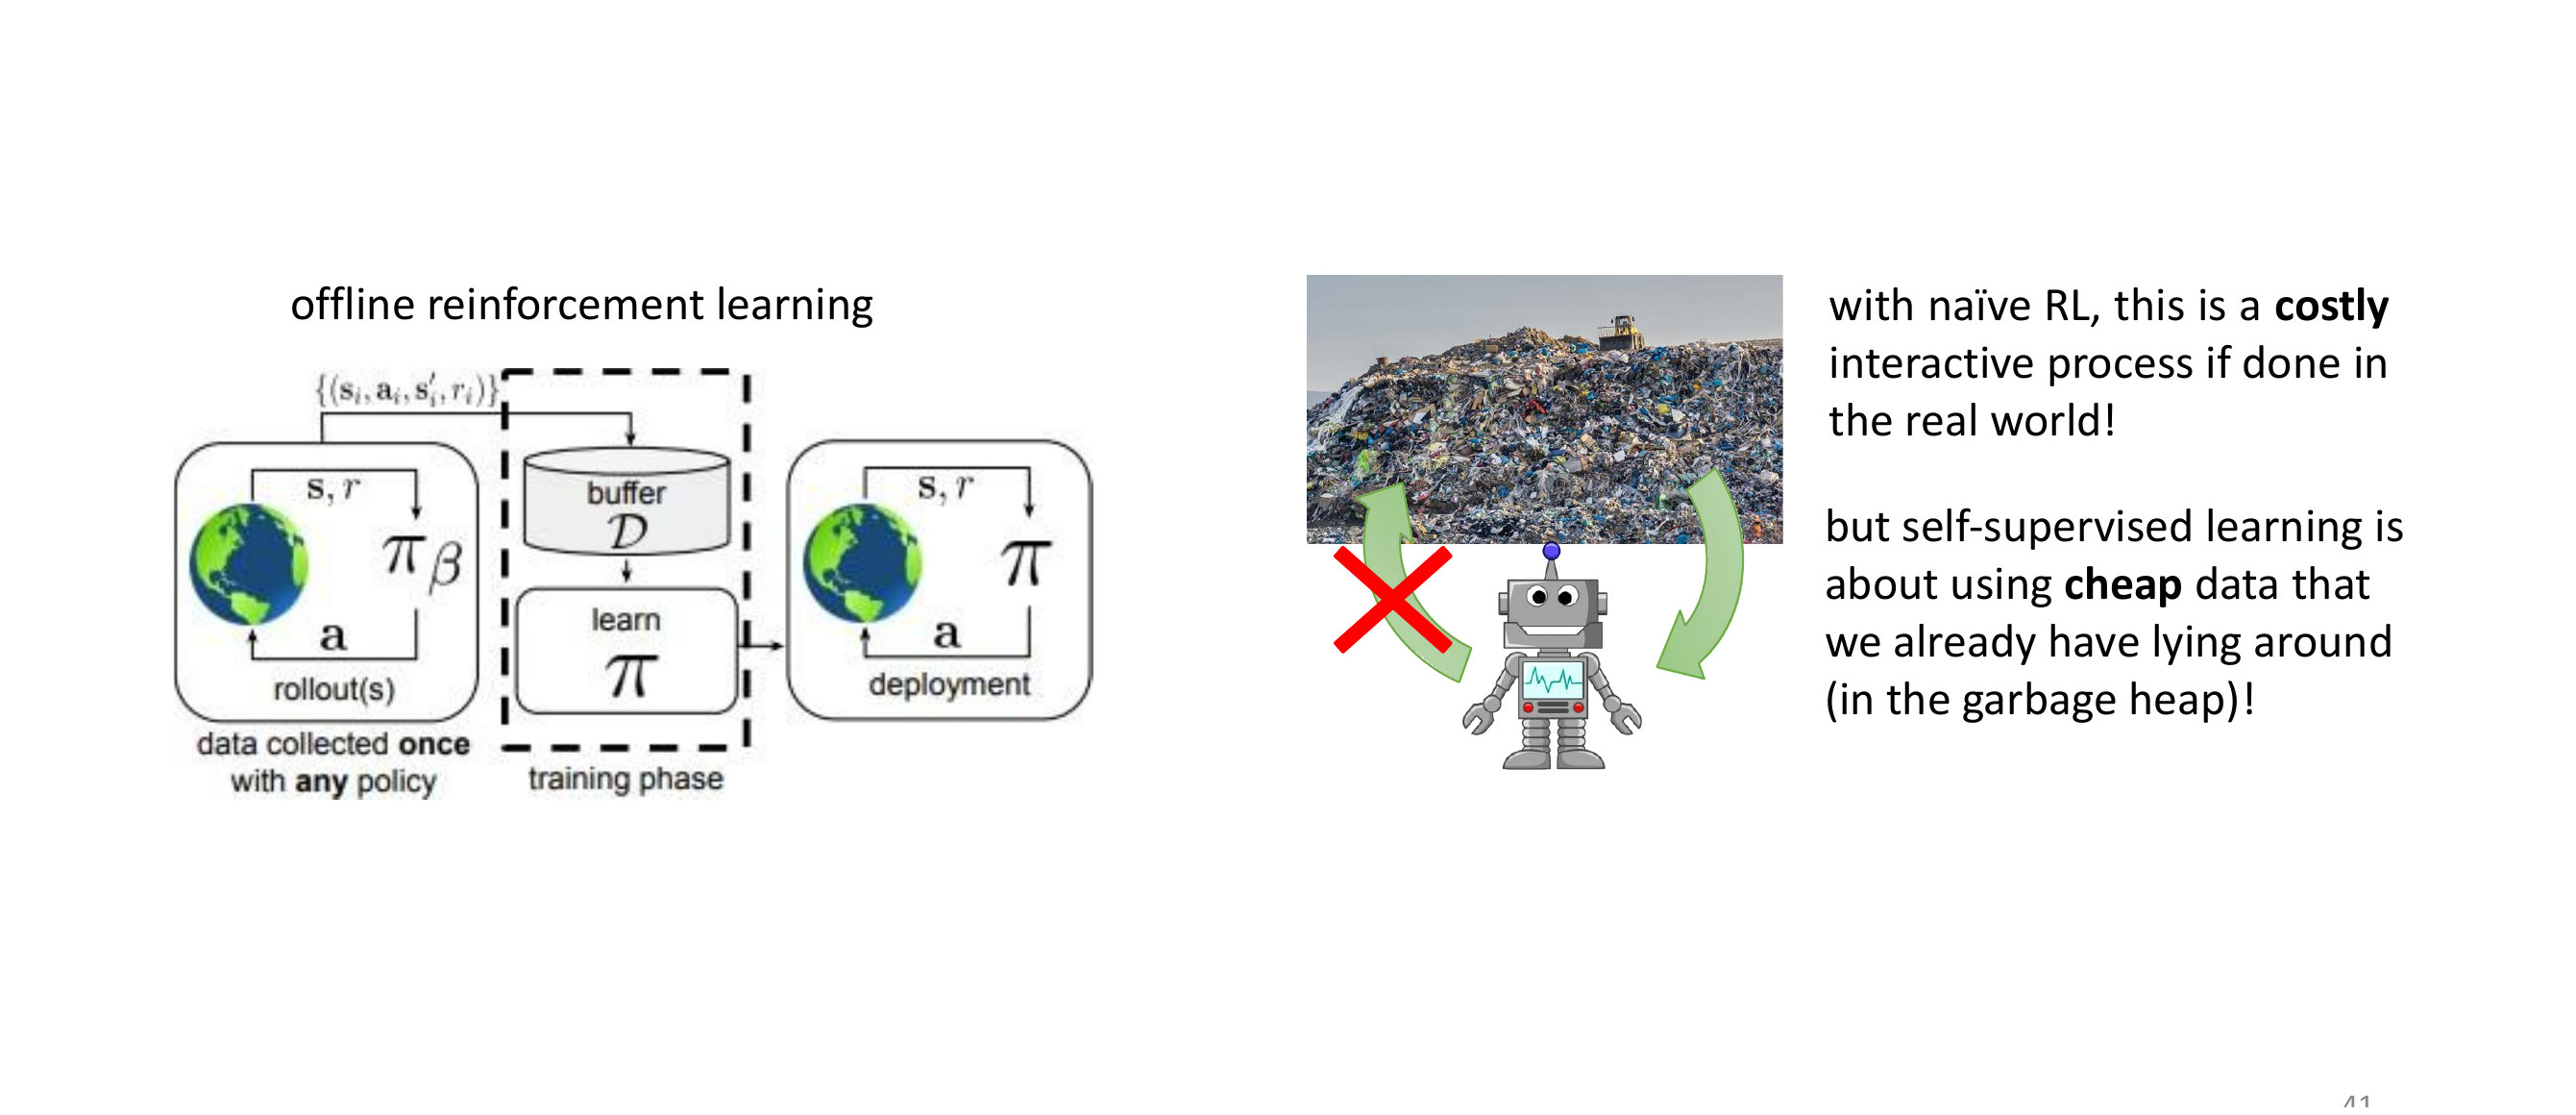
\includegraphics[width=\linewidth,height=0.82\textheight,keepaspectratio]{images/meta-rl-open/figures/rl-data-problem.jpg}
\end{frame}

% ---------------------------------------------------------------- Slide 63
\begin{frame}{The recipe}
\centering
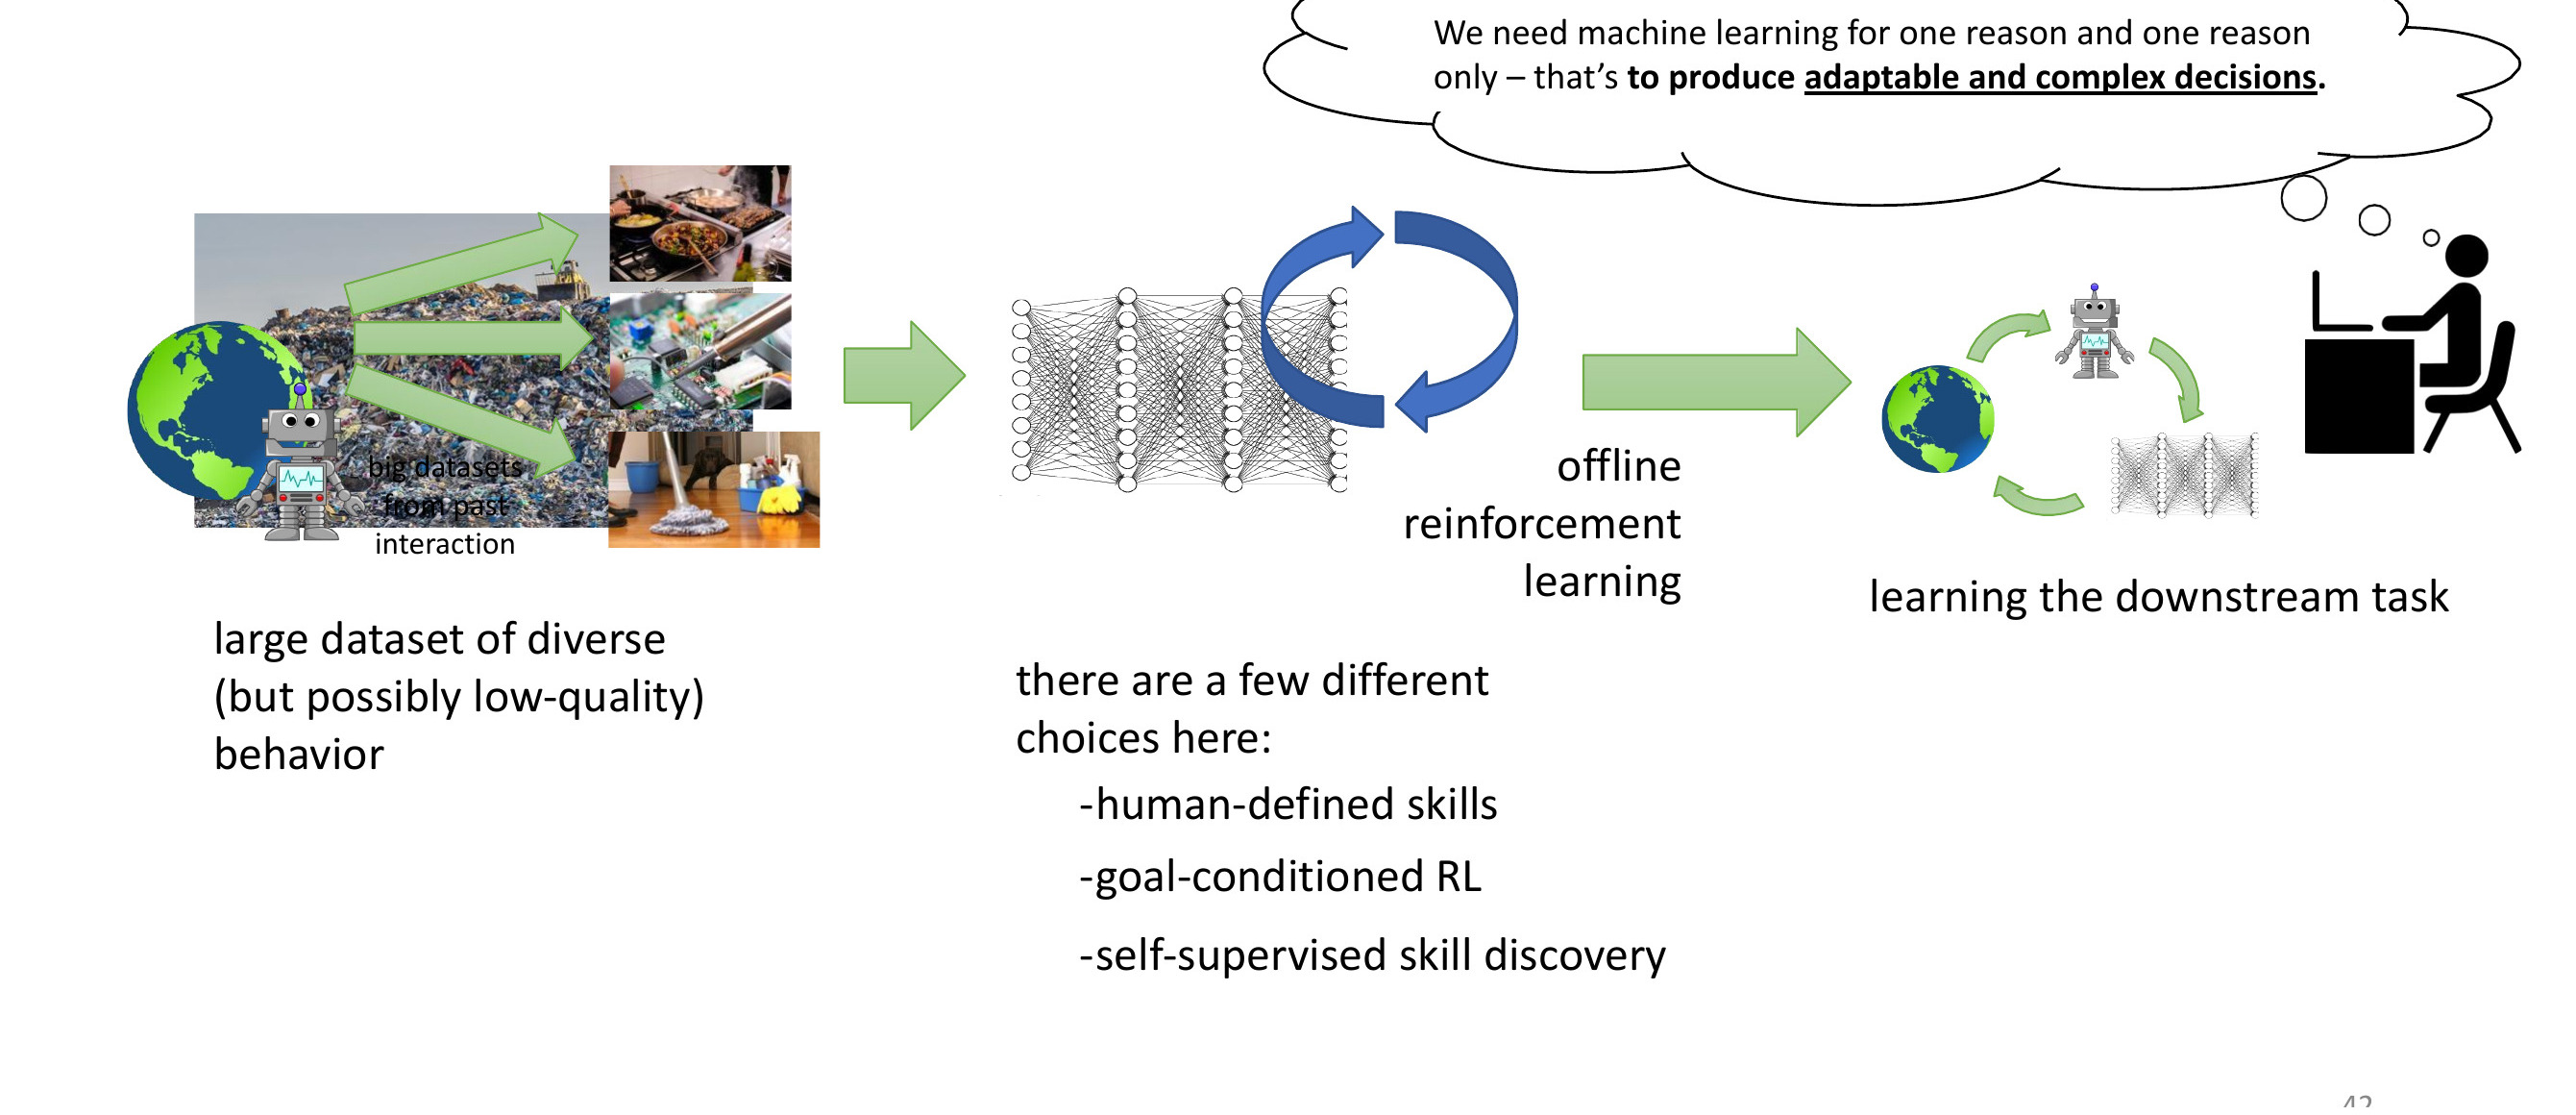
\includegraphics[width=\linewidth,height=0.82\textheight,keepaspectratio]{images/meta-rl-open/figures/recipe.jpg}
\end{frame}

% ---------------------------------------------------------------- Slide 64
\begin{frame}{Can we learn from offline data without well-defined tasks?}
\begin{columns}[c]
\begin{column}{0.4\textwidth}
\centering
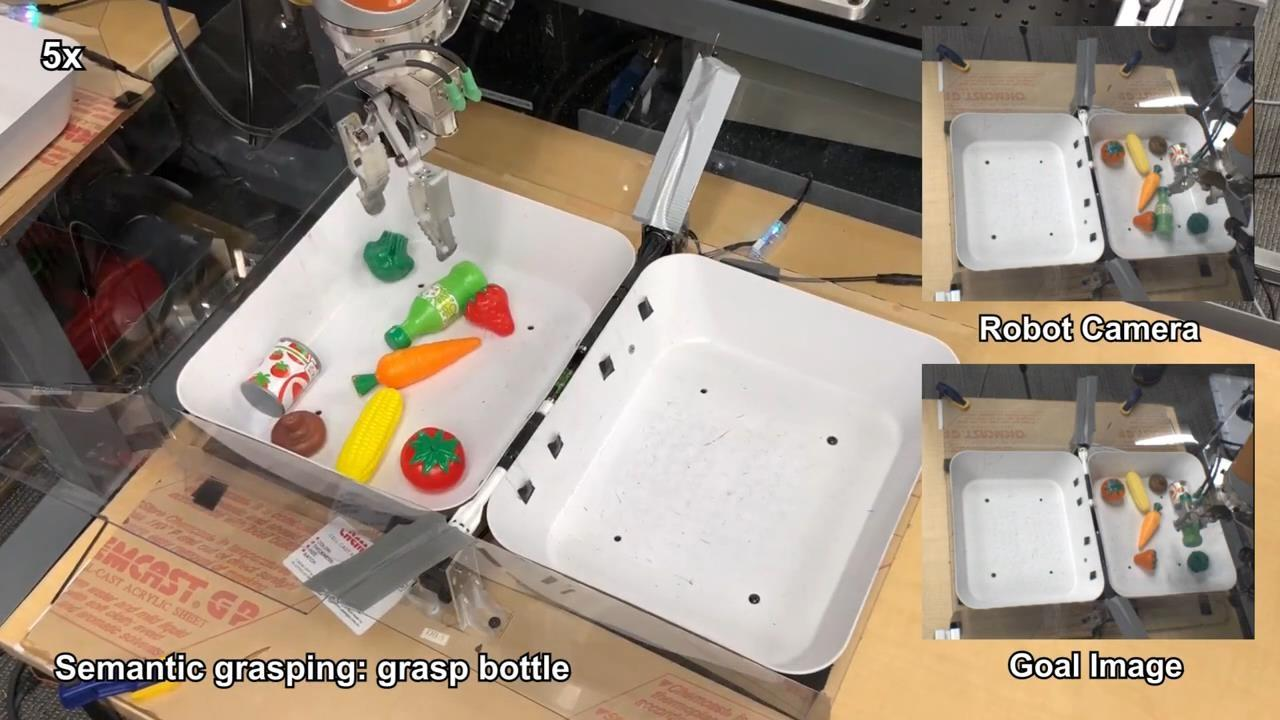
\includegraphics[width=\linewidth]{images/meta-rl-open/figures/actionable-models.jpg}
\end{column}
\begin{column}{0.6\textwidth}
\scriptsize
\begin{itemize}
    \item No reward function at all, task is defined entirely using a goal image
    \item Uses a conservative offline RL method designed for goal-reaching, based on CQL
    \item Works very well as an unsupervised pretraining objective
\end{itemize}
\vspace{0.2em}
\centering
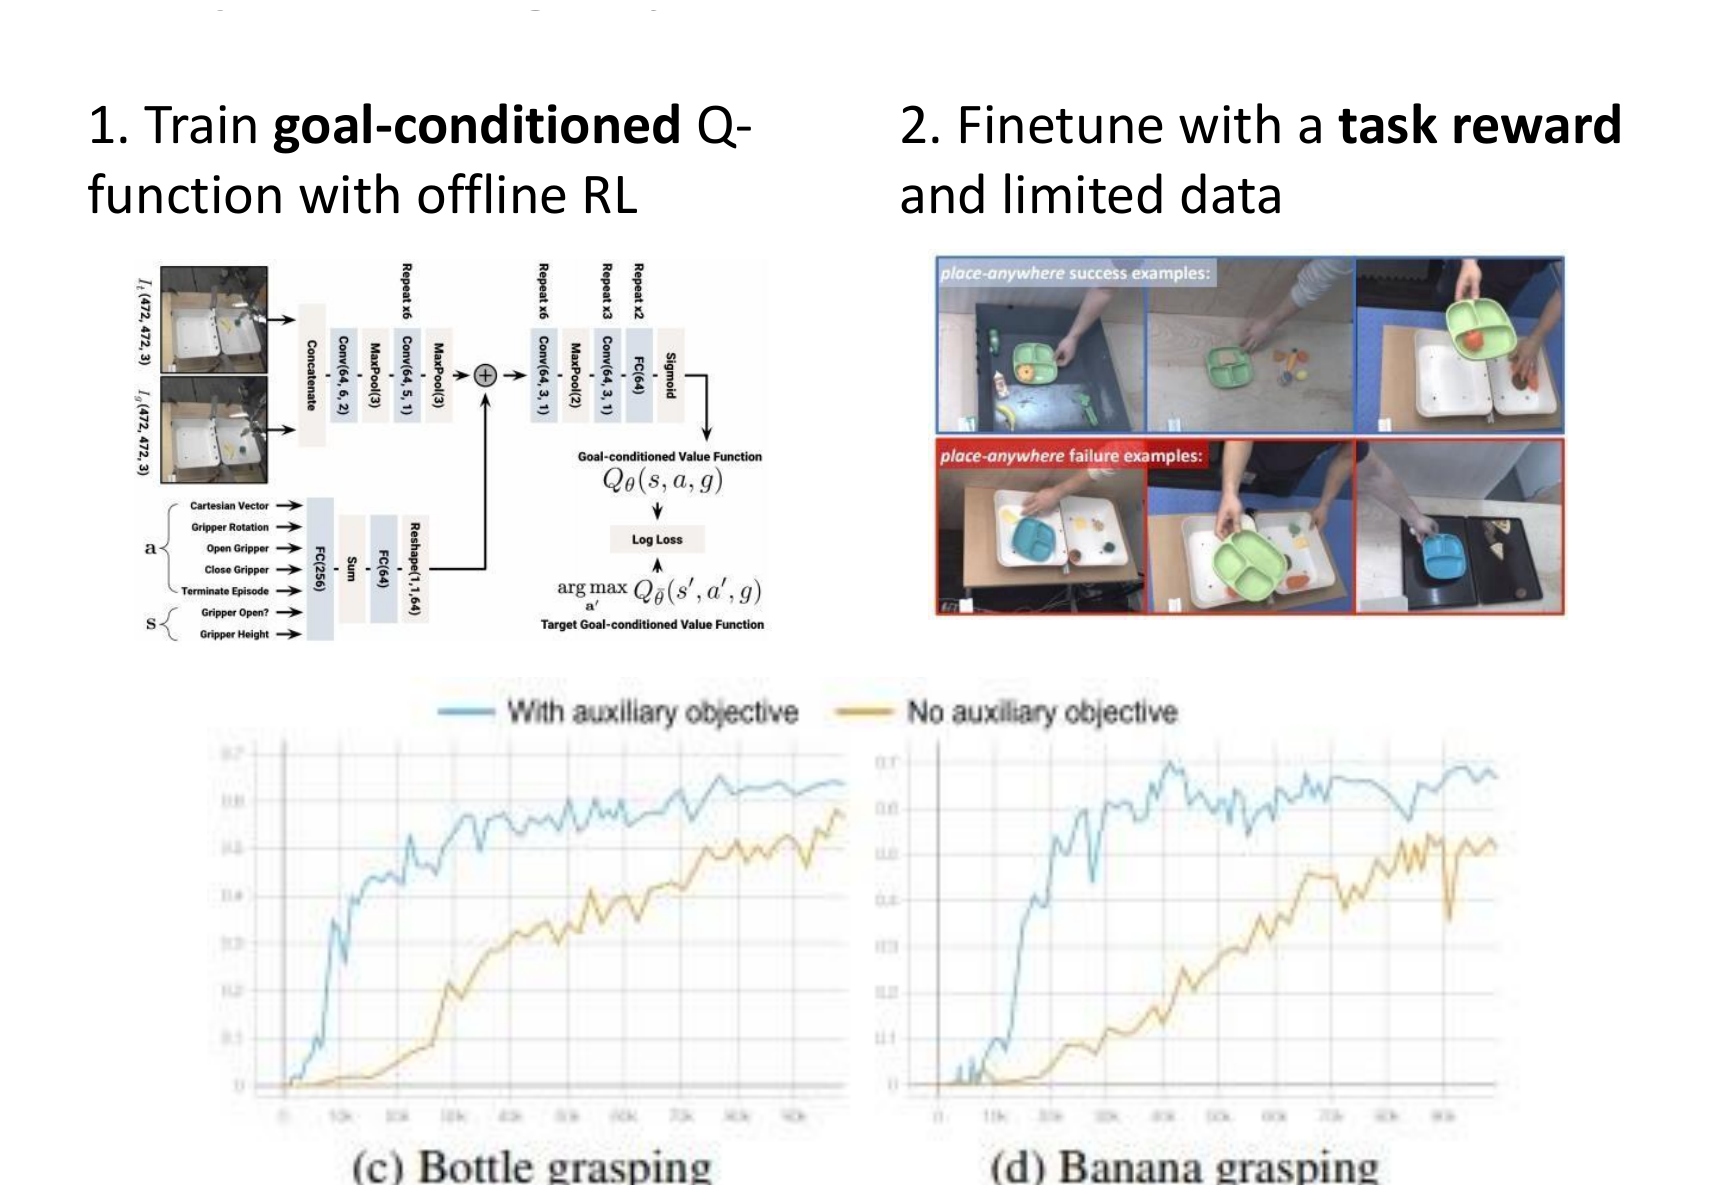
\includegraphics[width=\linewidth]{images/meta-rl-open/figures/actionable-right.png}
\end{column}
\end{columns}
\vfill
{\tiny Chebotar et al. Actionable Models: Unsupervised Offline Reinforcement Learning of
Robotic Skills. 2021.}
\end{frame}

% ---------------------------------------------------------------- Slide 65
\begin{frame}{Can offline RL train large language models?}
\begin{columns}[c]
\begin{column}{0.46\textwidth}
\centering
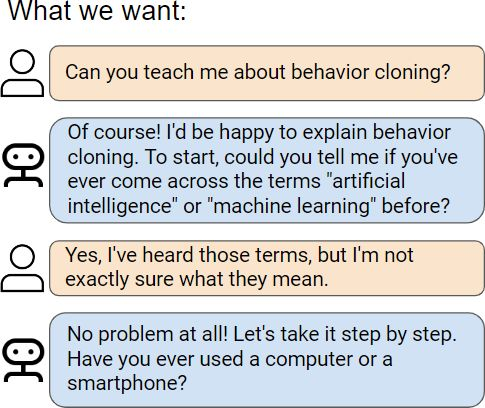
\includegraphics[width=\linewidth]{images/meta-rl-open/figures/llm-want.jpg}
\end{column}
\begin{column}{0.54\textwidth}
\centering
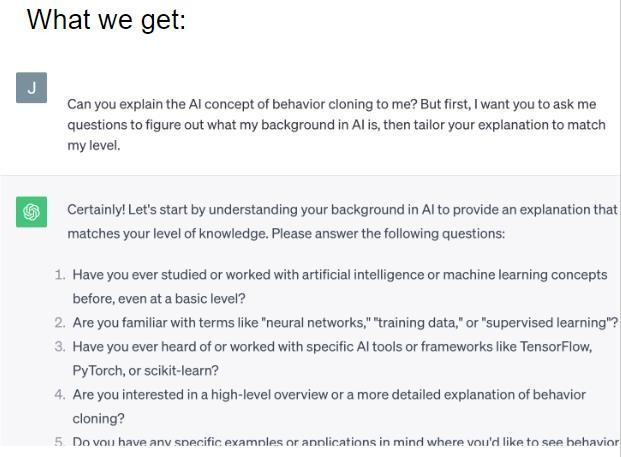
\includegraphics[width=\linewidth]{images/meta-rl-open/figures/llm-get.jpg}
\end{column}
\end{columns}
\end{frame}

% ---------------------------------------------------------------- Slide 66
\begin{frame}{Model-based offline RL for multi-turn dialogue}
\begin{columns}[c]
\begin{column}{0.62\textwidth}
\centering
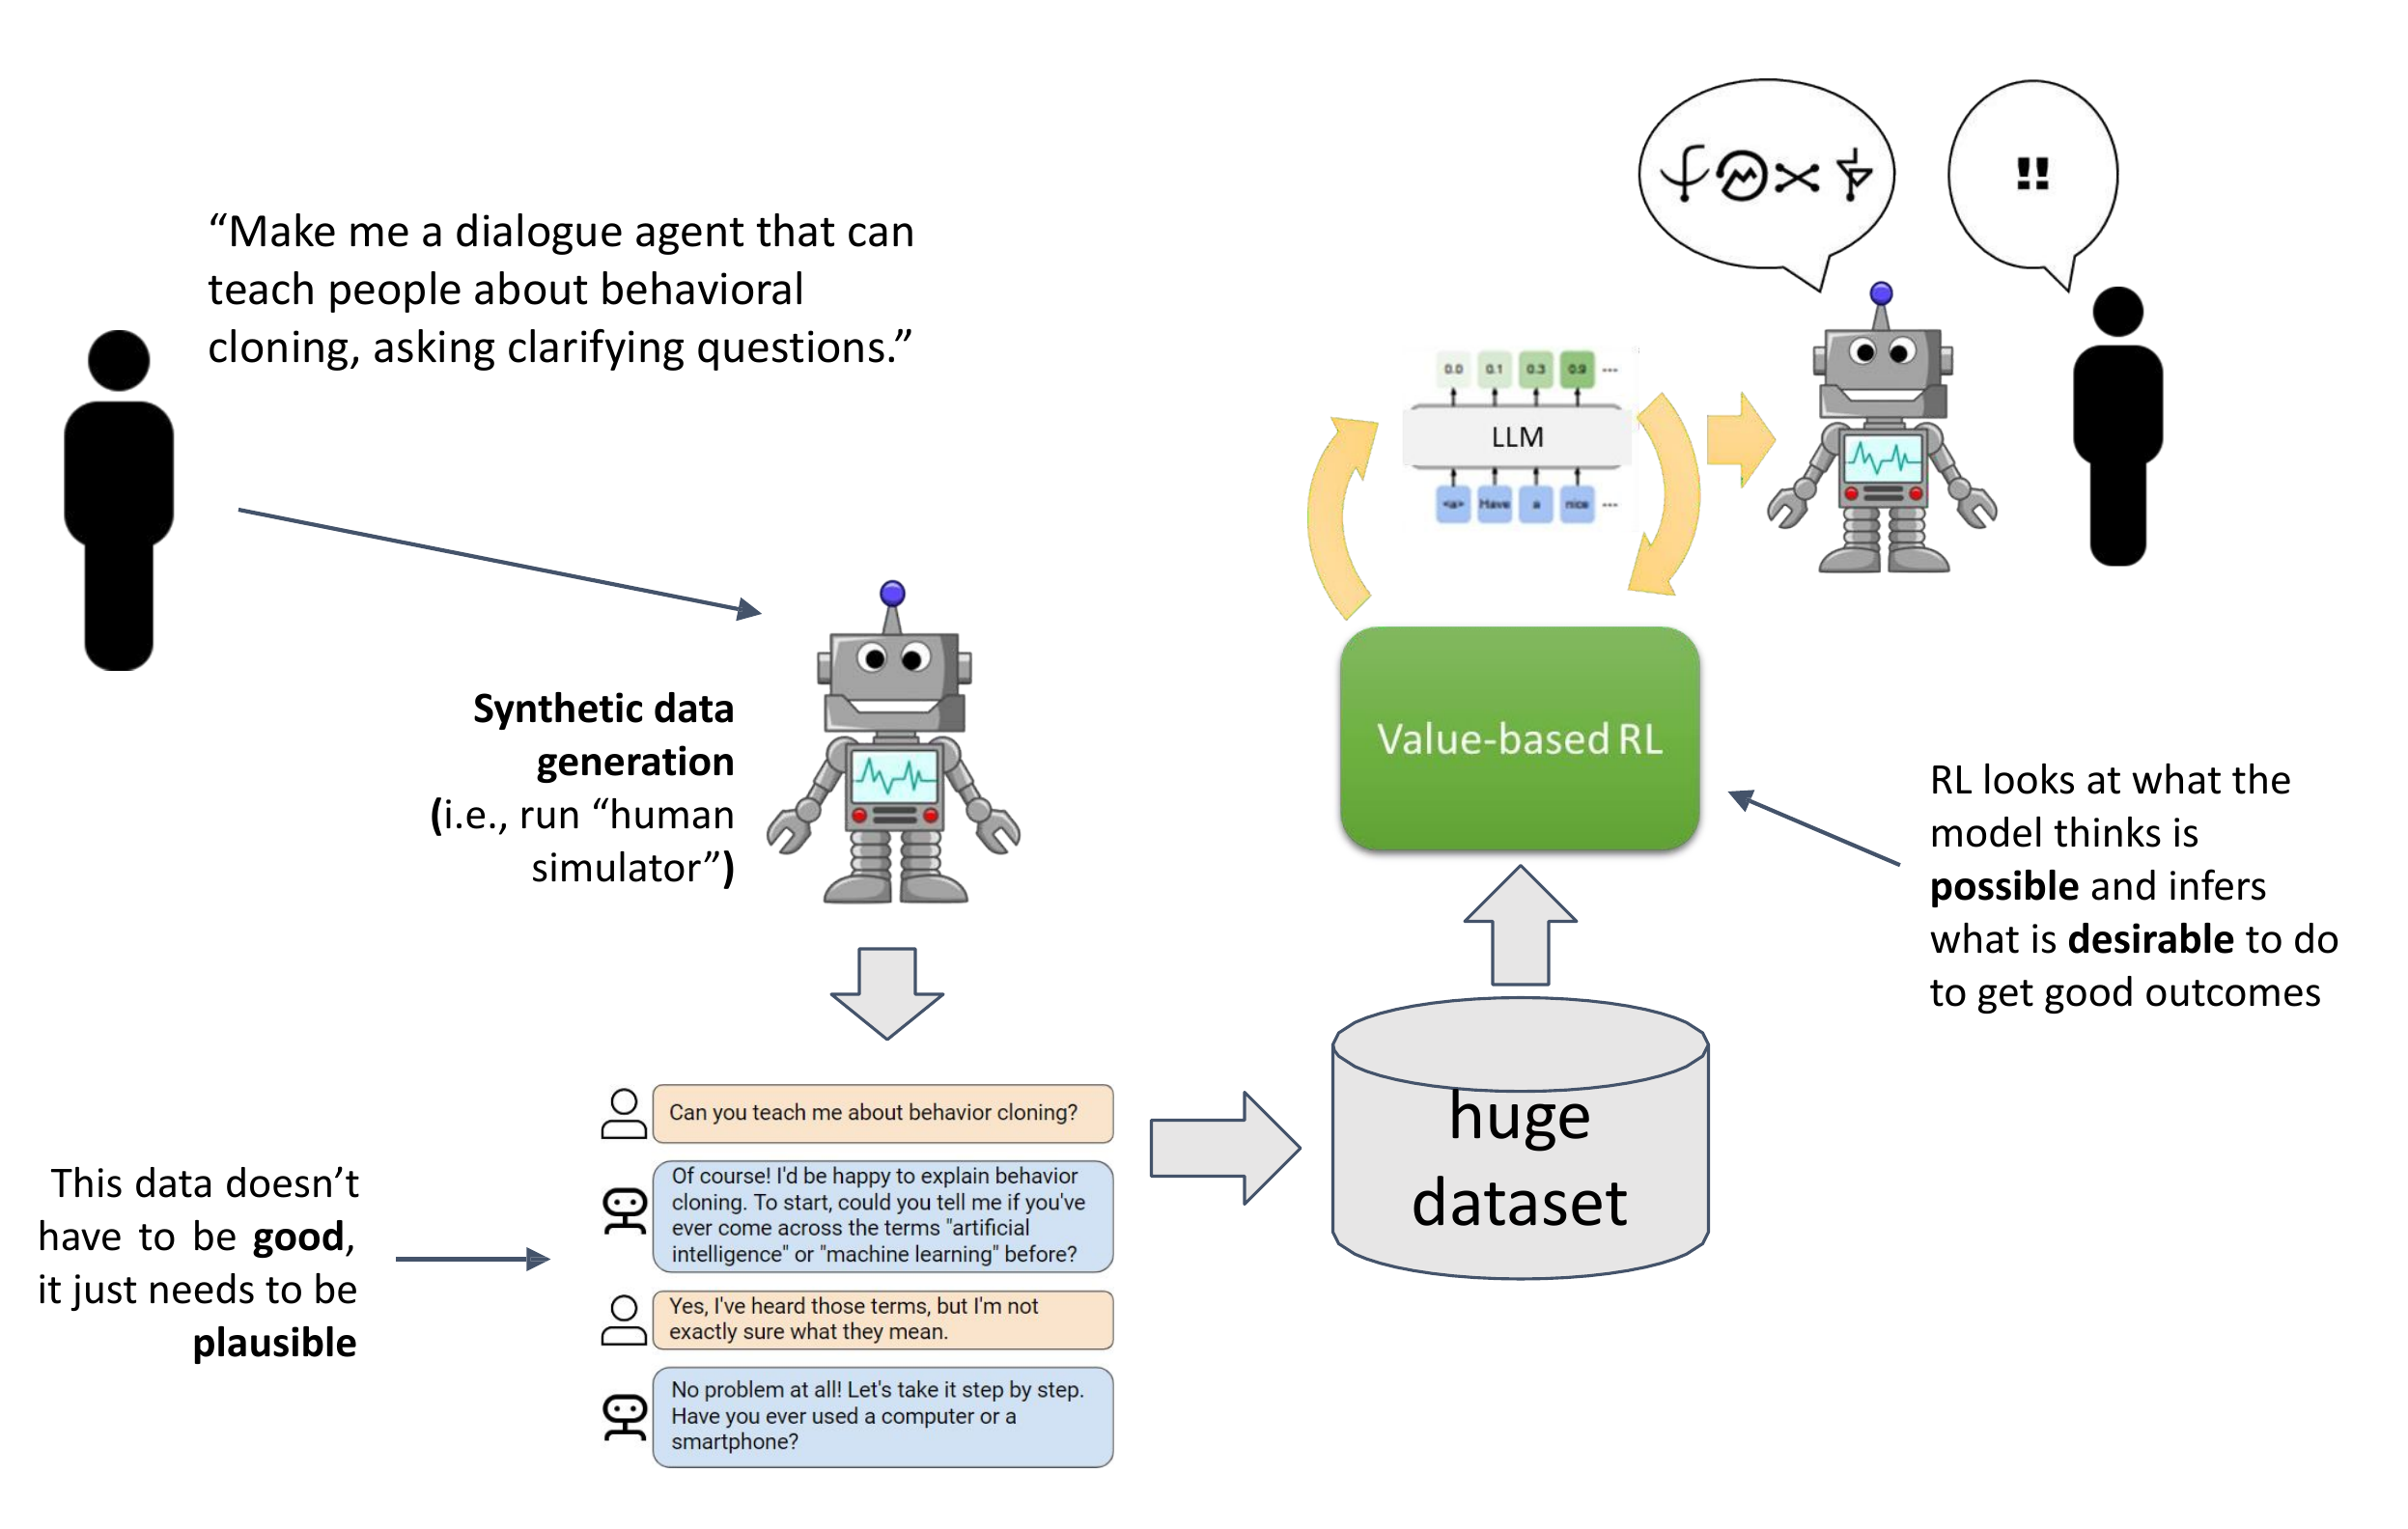
\includegraphics[width=\linewidth]{images/meta-rl-open/figures/dialogue-mb.png}
\end{column}
\begin{column}{0.38\textwidth}
\footnotesize
RL $+$ LLM is great for tasks that are easy for LLMs to simulate but hard for them to
perform optimally.
\vspace{0.5em}

With RL, instead of emulating humans, LLMs can learn to achieve desired outcomes using
their understanding of how humans behave.
\end{column}
\end{columns}
\vfill
{\tiny Hong, Levine, Dragan. Zero-Shot Goal-Directed Dialogue via RL on Imagined
Conversations. 2023.}
\end{frame}

% ---------------------------------------------------------------- Slide 67
\begin{frame}{Example: model-based RL for multi-turn dialogue}
\begin{columns}[c]
\begin{column}{0.5\textwidth}
\centering
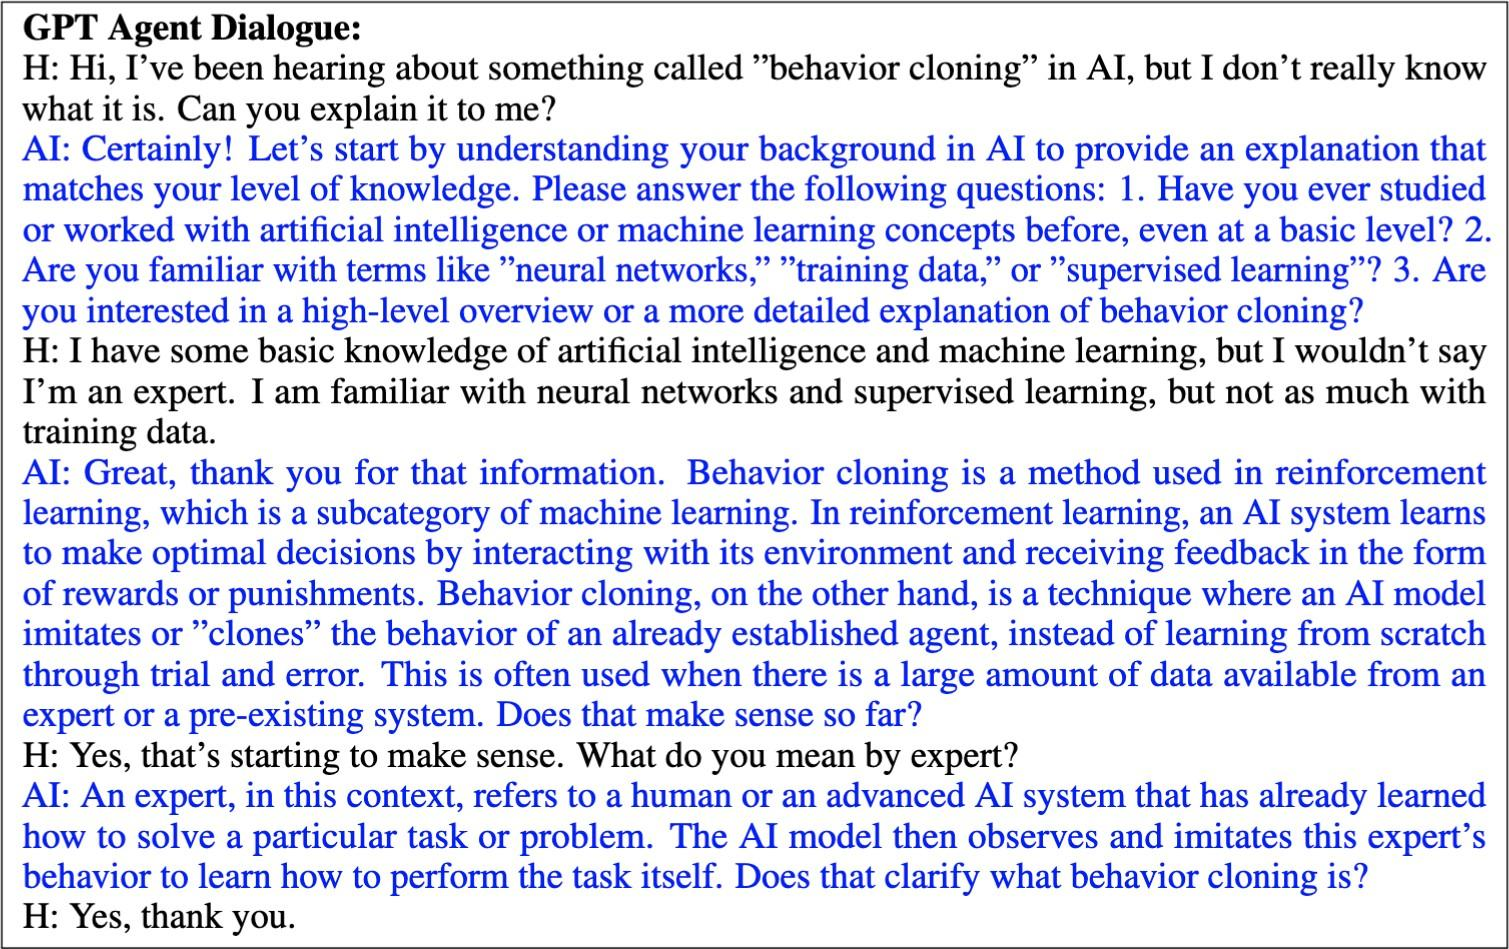
\includegraphics[width=\linewidth]{images/meta-rl-open/figures/dialogue-gpt.jpg}
\end{column}
\begin{column}{0.5\textwidth}
\centering
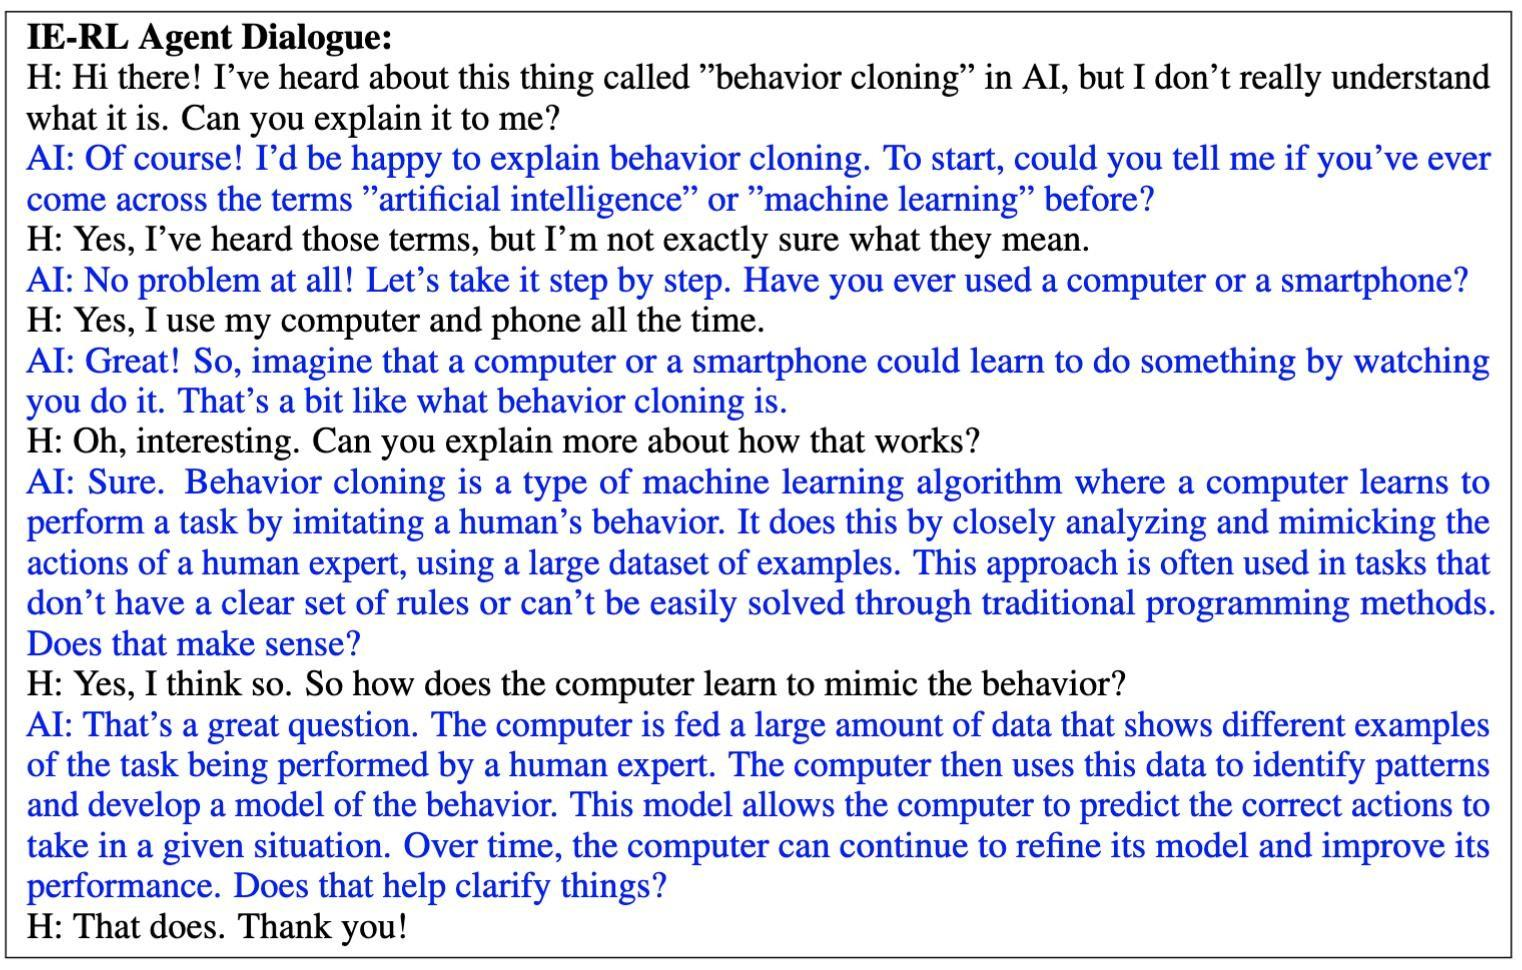
\includegraphics[width=\linewidth]{images/meta-rl-open/figures/dialogue-ierl.jpg}
\end{column}
\end{columns}
\vfill
{\scriptsize Hong, Levine, Dragan. Zero-Shot Goal-Directed Dialogue via RL on Imagined Conversations. 2023.}
\end{frame}
